\documentclass{standalone}
\usepackage{tikz}
\usepackage{hsbcommon}



\begin{document}
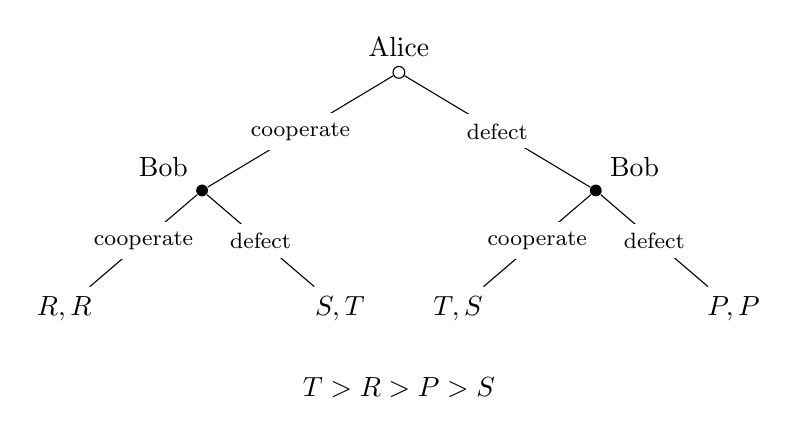
\begin{tikzpicture}[thin,
      level 1/.style={sibling distance=50mm},
      level 2/.style={sibling distance=35mm},
      level 3/.style={sibling distance=10mm},
      every circle node/.style={minimum size=1.5mm,inner sep=0mm}]
      
      \node[circle,draw,label=above:Alice] (root) {}
        child { node [circle,fill,label=above left:Bob] {}
          child { 
            node {$R,R$}
            edge from parent
              node[fill=white] {\footnotesize cooperate}}
          child { 
            node {$S,T$}
            edge from parent
              node[fill=white] {\footnotesize defect}}
          edge from parent
            node[fill=white] {\footnotesize cooperate}}
        child { node [circle,fill,label=above right:Bob] {}
          child { 
            node {$T,S$}
              edge from parent
                node[fill=white] {\footnotesize cooperate}}
          child { 
            node {$P,P$}
              edge from parent
                node[fill=white] {\footnotesize defect}}
           edge from parent
             node[fill=white] {\footnotesize defect}};

        \node at (0,-4cm) {$T>R>P>S$};
    \end{tikzpicture}
\end{document}
